\documentclass[a4paper]{article}

% Umlaute
\usepackage[T1]{fontenc}
% Wir wollen auch Umlaute schreiben
\usepackage[utf8]{inputenc}

\usepackage[ngerman]{babel}

\usepackage{graphicx}

\title{Blöder Titel}
\author{ich}
\date{\today}

% Ich komme immer zum Schluss!
\usepackage{hyperref}

\begin{document}
\section{Umlaute und aktuelle deutsche Rechtschreibung}
Fix Schwyz quäkt Jürgen blöd vom Paß.
The quick brown fox jumps over the lazy dog.

Binde immer \verb+\usepackage[T1]{fontenc}+, \verb+\usepackage[utf8]{inputenc}+ und \verb+\usepackage[ngerman]{babel}+ ein!

\section{Titel}
\maketitle % Titel

Siehe \verb+\author, \title+ und \verb+\date+

\section{Überschriften}

\section{Eine Überschrift}
\subsection{Eine Unterüberschrift}
\subsubsection{Eine Unterunterüberschrift}
\paragraph{Test}
\subparagraph{Sub-Test}

\tableofcontents

\section{Ein kurzer Abschnitt} \label{sec:Ein kurzer Abschnitt}
Auch gibt es niemanden, der den Schmerz an sich liebt, sucht oder wünscht, nur, weil er Schmerz ist, es sei denn, es kommt zu zufälligen Umständen, in denen Mühen und Schmerz ihm große Freude bereiten können. Um ein triviales Beispiel zu nehmen, wer von uns unterzieht sich je anstrengender körperlicher Betätigung, außer um Vorteile daraus zu ziehen? Aber wer hat irgend ein Recht, einen Menschen zu tadeln, der die Entscheidung trifft, eine Freude zu genießen, die keine unangenehmen Folgen hat, oder einen, der Schmerz vermeidet, welcher keine daraus resultierende Freude nach sich zieht? Auch gibt es niemanden, der den Schmerz an sich liebt, sucht oder wünscht, nur, weil er Schmerz ist, es sei denn, es kommt zu zufälligen Umständen, in denen Mühen und Schmerz ihm große Freude bereiten können. Um ein triviales Beispiel zu nehmen, wer von uns unterzieht sich je anstrengender körperlicher Betätigung, außer um Vorteile daraus zu ziehen? Aber wer hat irgend ein Recht, einen Menschen zu tadeln, der die Entscheidung trifft, eine Freude zu genießen, die keine unangenehmen Folgen hat, oder einen, der Schmerz vermeidet, welcher keine daraus resultierende Freude nach sich zieht?Auch gibt es niemanden, der den Schmerz an sich liebt, sucht oder wünscht, nur, 


\section{Querverweise}
Wie wir in Abschnitt~\ref{sec:Ein kurzer Abschnitt} gesehen haben, gilt ...

\url{tim.benedikt.herbstrith@univie.ac.at}

\href{mailto:tim.benedikt.herbstrith@univie.ac.at}{Schreib mir ein Mail!}

Springe im Dokument mit \verb+\usepackage{hyperref}+ (muss immer an letzter Stelle stehen!).

\section{Textschnitte}
Ich bin \textbf{fett.} \textit{kursiv,} \textsl{slanted,} \texttt{Schreibmaschine,}
\textsc{Kapitälchen}

\emph{Fix Schwyz} quäkt Jürgen blöd vom Paß.
The quick brown fox jumps over the lazy dog.

\textit{Fix Schwyz} quäkt Jürgen blöd vom Paß.

\itshape
Ab hier alles kursiv: Testtext

Fix Schwyz quäkt Jürgen blöd vom Paß.
The quick brown fox jumps over the lazy dog.
\upshape

\section{Bilder}

Hier kommt ein Bild (siehe Abb.~\ref{im:Bibel})

\begin{figure}
\begin{center}
    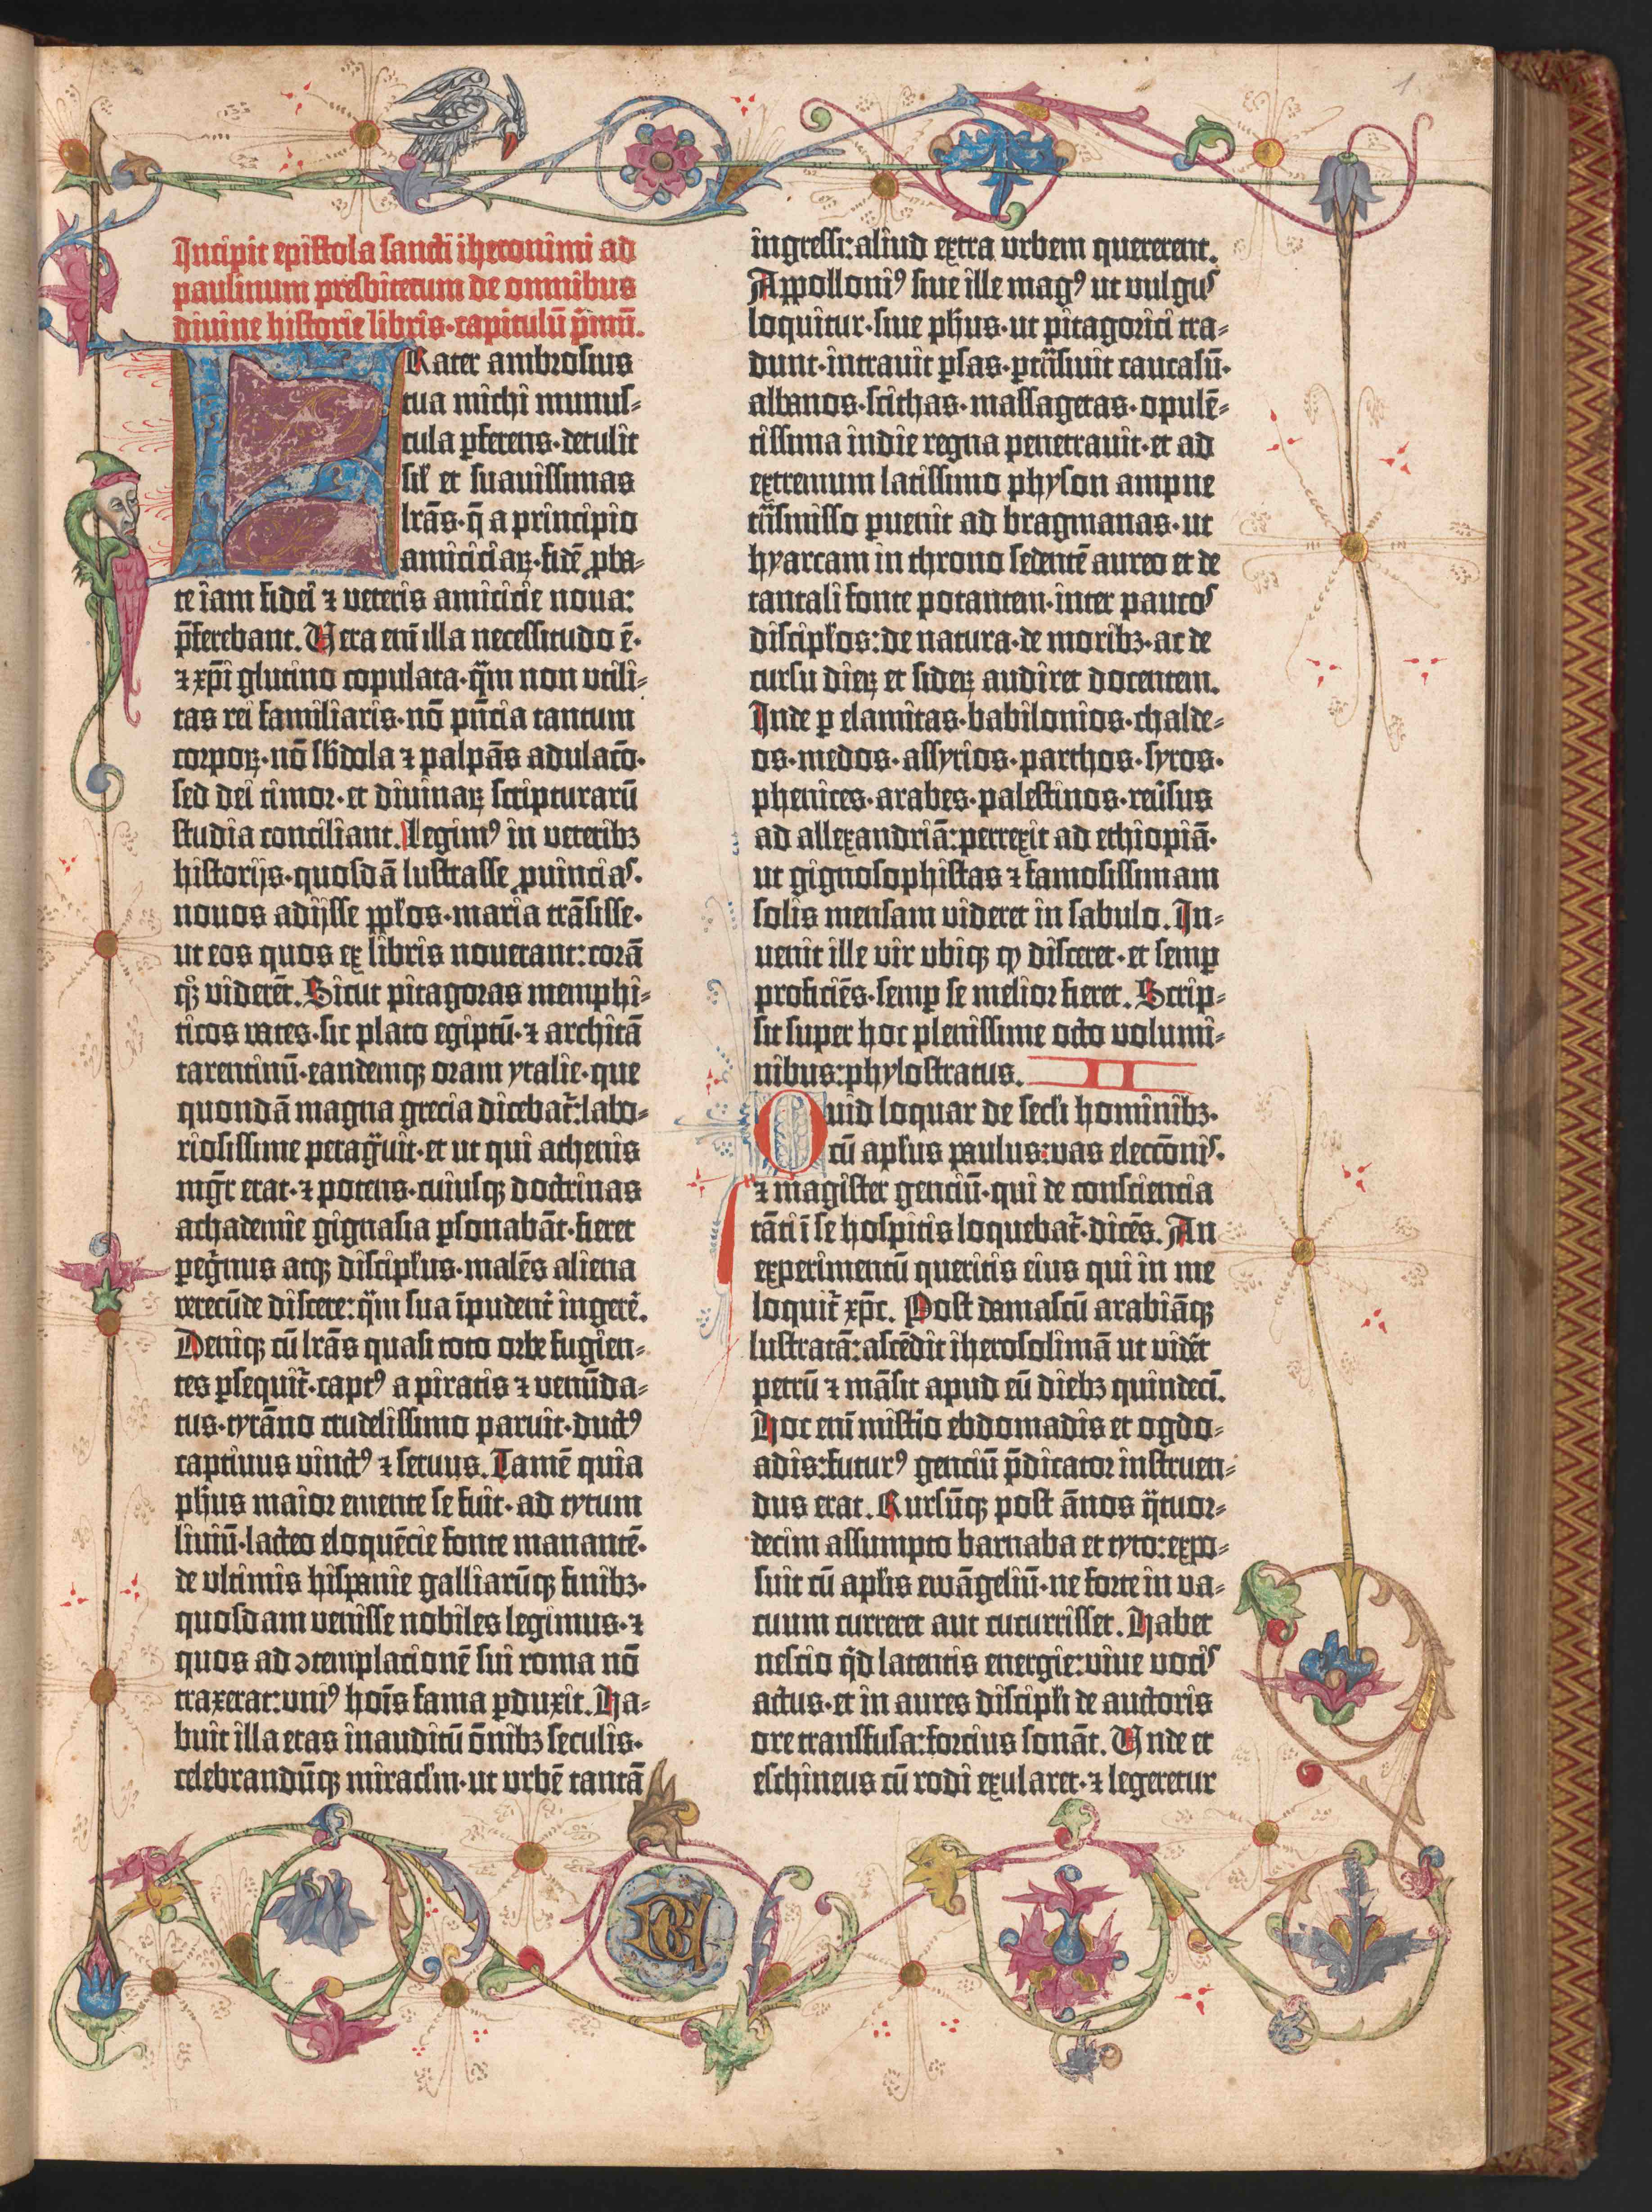
\includegraphics[width=0.5\linewidth]{./res/gutenberg.jpg}
\caption{Gutenberg Bibel}
\label{im:Bibel}
\end{center}
\end{figure}

Hier geht es weiter.
\listoffigures

Binde \verb+\usepackage{graphicx}+ ein.

\section{Tabellen}
Hier kommt Text.
\begin{table}[tbp]
\begin{center}
\begin{tabular}{|p{2cm}|c r|}
\hline
links    &    mitte    &    rechts\\
\hline
Zweile   &    Zwei     &    !\\
Donau\-dampf\-schiff\-fahrts\-ge\-sell\-schaft&&\\
\hline
\hline
\end{tabular}
\caption{Eine Tabelle}
\label{tab:Tabelle}
\end{center}
\end{table}
Und noch mehr Text, der auf die Tabelle verweist (siehe Tab.~\ref{tab:Tabelle}).
\listoftables
\end{document}






